% Consolidated subtraction benchmark (FLOW_NOTES.md, "Consolidated benchmark").
% Build: cd docs/flow/bench/slides && ~/pyext/tectonic_env/bin/tectonic bench_deck.tex
% Tables: tables/*.tex, written by scripts/flow/bench_tables.py from the CSVs
% in docs/flow/bench; figures: docs/flow/bench/*.png.
\documentclass[aspectratio=169,10pt]{beamer}
\usetheme{default}
\usefonttheme{professionalfonts}
\setbeamertemplate{navigation symbols}{}
\setbeamertemplate{footline}{%
  \hspace{1em}\textcolor{gray}{\tiny Flow matching vs UVCGAN-S: background subtraction benchmark, 2026-09-28}%
  \hfill\textcolor{gray}{\tiny\insertframenumber}\hspace{1em}\vspace{0.6em}}
\setbeamerfont{frametitle}{size=\large,series=\bfseries}
\setbeamercolor{frametitle}{fg=black}
\setbeamertemplate{itemize items}{\textbullet}
\setbeamersize{text margin left=0.9em,text margin right=0.9em}

\usepackage{booktabs}
\usepackage{graphicx}
\usepackage{xcolor}
\usepackage{array}
\graphicspath{{../}}

\definecolor{cUV}{HTML}{1f77b4}
\definecolor{cArea}{HTML}{7f7f7f}
\definecolor{cUnp}{HTML}{2ca02c}
\definecolor{cPai}{HTML}{ff7f0e}
\definecolor{cJnt}{HTML}{d62728}
\newcommand{\uv}{\textcolor{cUV}{\textbf{UVCGAN-S}}}
\newcommand{\area}{\textcolor{cArea}{\textbf{Area}}}
\newcommand{\unp}{\textcolor{cUnp}{\textbf{unpaired FM}}}
\newcommand{\pai}{\textcolor{cPai}{\textbf{paired FM}}}
\newcommand{\jnt}{\textcolor{cJnt}{\textbf{joint FM}}}
\newcommand{\Bh}{\hat B}
\newcommand{\Sh}{\hat S}
\newcommand{\snote}[1]{{\scriptsize\textcolor{gray}{#1}}}

\begin{document}
% Slide bodies of bench_deck.tex. Numbers: docs/flow/bench/*.csv (seed means
% of 3 unless stated); tables/*.tex are written by scripts/flow/bench_tables.py.

% ---------------------------------------------------------------- 1
\begin{frame}{Background subtraction $M = S + B$: predict $B$ alone, or $B$ and $S$ together?}
\small
\textbf{Question.} Flow matching (FM) from the mixture $M$: predict only the background and read
$\Sh = M - \Bh$, or predict both components? And what does training each mixture with its
\emph{own} background (simulation truth) change? Judged on individual jets, not only on the
average energy resolution.

\vspace{0.4em}
\textbf{Controlled comparison.} Three FM arms with the same network (the UVCGAN-S generator),
the same 633k training mixtures and 2 h on one A6000, 3 seeds each; the published
\uv{} (${\sim}$105 h of training) and \area{} subtraction on the same 20k PYTHIA+HIJING and
20k JEWEL+HIJING events; the paper's jet analysis rebuilt.

\vspace{0.4em}
\textbf{Answer} (PYTHIA val, R = 0.4, $20 < p_T < 30$ GeV):
\begin{itemize}\setlength\itemsep{0.15em}
\item \textbf{No FM arm is as faithful as \uv{}} (scale 0.98, 3\% fakes, substructure
  distributions 2-7$\times$ closer than the best FM arm's). After a frozen calibration the jet
  resolution is the same for \uv{}, \unp{} and \pai{} (0.150-0.154); \jnt{} is 5-7\% worse.
\item \textbf{Predicting $B$ alone loses part of the jet core}: 12-25\% of the energy in towers
  with $S > 10$ GeV goes into $\Bh$. \pai{}: jet scale 0.83. \unp{} looks unbiased (0.99) only
  because a soft floor adds 112 GeV per event: 15\% fake jets at 14-20 GeV.
\item \textbf{Predicting $B$ and $S$ keeps the hard core} ($\le$3\% lost) but drops soft signal:
  scale 0.91 at R = 0.4 (0.99 at R = 0.2), efficiency 0.88 at 14-20 GeV, 10$\times$ larger seed
  spread.
\item \textbf{Pairing} cuts the per-tower error 3$\times$ and fakes 30$\times$ and gives the
  smallest per-jet errors of girth, $z_{lead}$ and $r_g$ of all models, but does not fix the
  jet scale. It needs simulation truth.
\end{itemize}
\end{frame}

% ---------------------------------------------------------------- 2
\begin{frame}{Setup: one network and one budget; only the pairing and the outputs change}
\scriptsize
\begin{tabular}{@{}l l p{0.33\textwidth} p{0.13\textwidth} p{0.17\textwidth}@{}}
\toprule
arm & flow & training pairs & loss & signal readout \\
\midrule
\unp & $M \to B$ & minibatch exact OT: real mixtures $\leftrightarrow$ independent HIJING events & CFM MSE & $\Sh = M - \Bh$ \\
\pai & $M \to B$ & each mixture with \emph{its own} background ($B = M - S$, bookkeeping) & CFM MSE & $\Sh = M - \Bh$ \\
\jnt & $(M, 0) \to (B, S)$ & each mixture with its own $(B, S)$ & mean$_B$ + mean$_S$, weight 1 each & direct $\Sh$; $M - \Bh$ (reported separately) \\
\bottomrule
\end{tabular}

\vspace{0.5em}
\begin{columns}[T]
\column{0.5\textwidth}
\textbf{Common to the three FM arms}
\begin{itemize}\setlength\itemsep{0.05em}
\item velocity net: the UVCGAN-S generator (ViT-ModNet, 32.3M parameters), time added to its style token
\item $\log(E + 0.1)$ standardised; straight path, $\sigma = 0$; deterministic transports, not samplers
\item Adam $2\cdot10^{-4}$, batch 256, EMA 0.9999, \textbf{2 h on one A6000}, 3 seeds (32k updates)
\item the same 633k real embedded training mixtures
\item one checkpoint per run: lowest val cone resolution (4 Euler steps, $M - \Bh$)
\item solves: 4 Euler steps and midpoint 32 NFE (= 64 NFE on val); each readout shown at its val-preferred solve, both in the backup
\end{itemize}
\column{0.5\textwidth}
\textbf{References on the same events}
\begin{itemize}\setlength\itemsep{0.05em}
\item \uv{} published, one pass: batch 4, 800k updates (${\sim}$105 h); GAN + cycle + \texttt{idt-aa}, i.e.\ also \emph{supervised} on synthetic sums $B + S$
\item \area{}: FastJet $p_T - \rho A$, no substructure. ICS unavailable (no fjcontrib)
\end{itemize}
\textbf{Evaluation}
\begin{itemize}\setlength\itemsep{0.05em}
\item development: 20k PYTHIA+HIJING val; frozen test: 20k JEWEL+HIJING
\item paper's analysis rebuilt: FastJet anti-$k_T$, $R$ = 0.2/0.4/0.5, towers as constituents, one-to-one matching $\Delta R < 0.75R$, soft drop $z_{cut}$ 0.1, $\beta$ 0
\item raw outputs primary; frozen calibration from val events 10k-20k
\item \pai{} and \jnt{} use simulation truth: a supervised reference, not an upper bound
\end{itemize}
\end{columns}
\end{frame}

% ---------------------------------------------------------------- 3
\begin{frame}{Cost: 2 h per flow on one GPU; only unpaired FM reaches 3.70 GeV}
\vspace{-0.4em}
\begin{center}
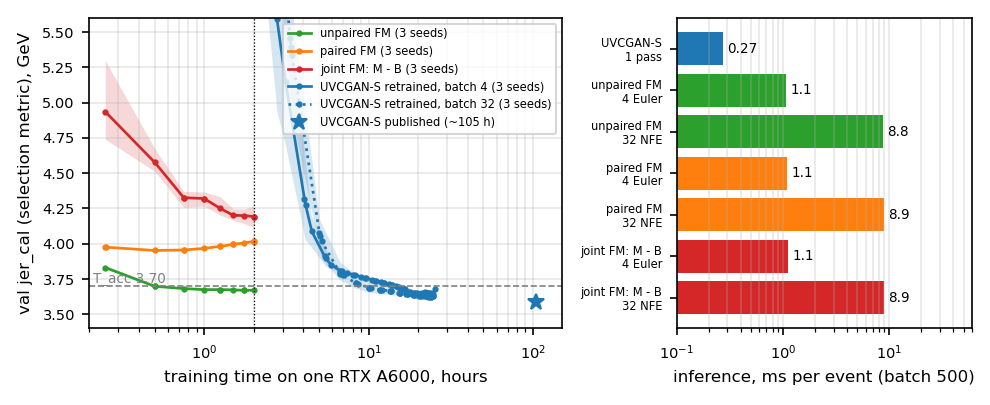
\includegraphics[width=0.7\textwidth]{bench_cost.png}
\end{center}
\vspace{-1.1em}
\scriptsize
\begin{tabular}{lrrrrrrr}
\toprule
 & best val res. & at 2 h & h to 3.70 & updates/s & peak GB & ms/event, 4 NFE & 32 NFE \\
\midrule
\unp & 3.67$\pm$0.01 & 3.67$\pm$0.01 & 0.5/0.5/0.5 & 4.45$\pm$0.03 & 19.1 & 1.08 & 8.8 \\
\pai & 3.95$\pm$0.00 & 4.02$\pm$0.01 & --/--/-- & 4.55$\pm$0.03 & 18.1 & 1.10 & 8.9 \\
\jnt & 4.15$\pm$0.04 & 4.19$\pm$0.08 & --/--/-- & 4.52$\pm$0.02 & 18.1 & 1.11 & 8.9 \\
\uv{} retrained, batch 4 & 3.64$\pm$0.02 & 7.44$\pm$0.70 & 15/17/17 & -- & -- & -- & -- \\
\uv{} retrained, batch 32 & 3.62$\pm$0.03 & 8.29$\pm$0.24 & 8.4/8.6/15 & -- & -- & -- & -- \\
\uv{} published (${\sim}$105 h) & 3.59 & -- & -- & -- & -- & 0.27 (1 pass) & -- \\
\bottomrule
\end{tabular}
\par\vspace{0.15em}\snote{One RTX A6000 each; flows 2 h, \uv{} retrained 24 h. val res.: the selection metric (calibrated cone resolution, GeV), seed mean $\pm$ half range. h to 3.70 (T\_acc = published + 3\%): first confirmed checkpoint, per seed. Inference: batch 500. The joint arm's second output costs $<$1\%.}

\end{frame}

% ---------------------------------------------------------------- 4
\begin{frame}{Jets: the background-only flows lose energy or hide the loss under fakes}
\vspace{-0.5em}
\begin{center}
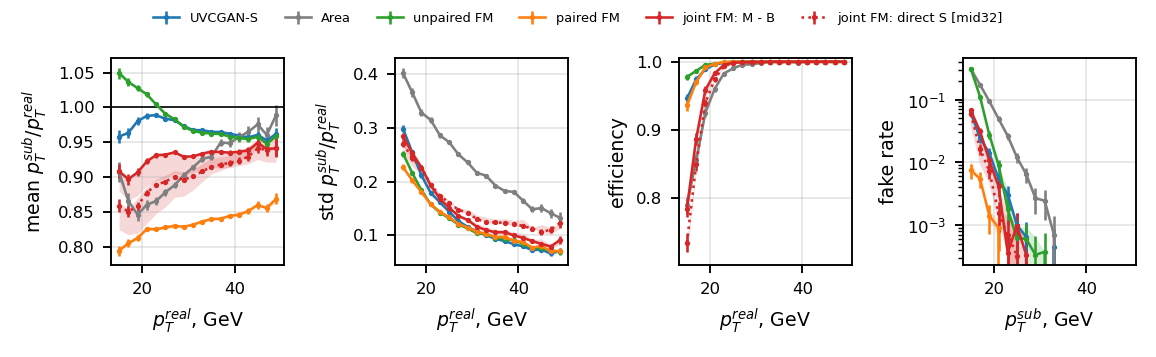
\includegraphics[width=0.8\textwidth]{bench_jets_R04_val.png}
\end{center}
\vspace{-1.3em}
\scriptsize
\begin{tabular}{lrrrrrr}
\toprule
 & scale & resolution & RMSE, GeV & res.\ (frozen cal.) & eff.\ 14-20 & fake 14-20 \\
\midrule
\uv & 0.982 & 0.144 & 3.59 & 0.153 & 0.972 & 0.030 \\
\area & 0.881 & 0.269 & 7.37 & 0.261 & 0.865 & 0.192 \\
\unp & 0.993(1) & 0.133 & 3.33(1) & 0.150 & 0.988 & 0.146(1) \\
\pai & 0.828(2) & 0.133 & 5.51(5) & 0.154 & 0.968(1) & 0.005 \\
\jnt, $M - \Bh$ & 0.912(16) & 0.153(1) & 4.41(19) & 0.161(3) & 0.881(6) & 0.029(3) \\
\jnt, direct $\Sh$ (32) & 0.884(22) & 0.163(1) & 5.02(35) & 0.164(1) & 0.846(6) & 0.020(4) \\
\snote{stat.\ error} & \snote{0.001} & \snote{0.001} & \snote{0.03} & \snote{0.001} & \snote{0.004} & \snote{0.003} \\
\bottomrule
\end{tabular}
\par\vspace{0.15em}\snote{Matched jets, $20 < p_T^{real} < 30$ GeV; efficiency ($p_T^{real}$), fake rate ($p_T^{sub}$), GeV. Raw, 4 Euler steps; (32): 32 NFE. Seed mean of 3; (n): seed half range in the last digit.}


\vspace{-0.1em}
{\scriptsize \textbf{The radius separates the failure modes.} Scale at $R$ = 0.2 / 0.4 / 0.5:
\uv{} 0.99 / 0.98 / 0.98; \unp{} 0.88 / 0.99 / 1.10 (its floor fills larger cones; 67\% fakes
at $R = 0.5$); \pai{} 0.82 / 0.83 / 0.85; \jnt{} 0.99 / 0.91 / 0.89 (core kept, periphery lost).}
\end{frame}

% ---------------------------------------------------------------- 5
\begin{frame}{Substructure: UVCGAN-S matches the distributions, paired FM the single jets}
\vspace{-0.6em}
\begin{center}
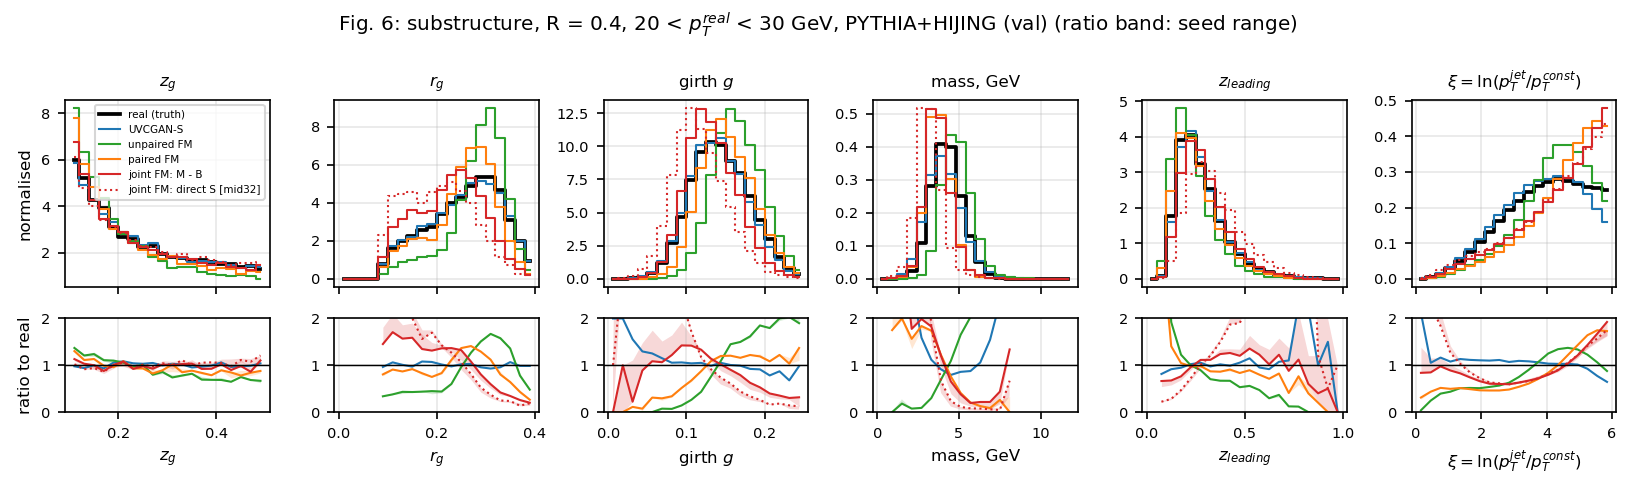
\includegraphics[width=0.8\textwidth]{bench_fig6_val.png}
\end{center}
\vspace{-1.4em}
\begin{center}
\footnotesize
\setlength{\tabcolsep}{4pt}
\begin{tabular}{lrrrrrrrrrrrr}
\toprule
 & \multicolumn{6}{c}{per-jet RMSE / $\sigma_{truth}$} & \multicolumn{6}{c}{distribution $W_1$ / $\sigma_{truth}$} \\
\cmidrule(lr){2-7}\cmidrule(lr){8-13}
 & $g$ & $m$ & $z_{lead}$ & $p_T^D$ & $z_g$ & $r_g$ & $g$ & $m$ & $z_{lead}$ & $p_T^D$ & $z_g$ & $r_g$ \\
\midrule
\uv & 0.60 & 1.16 & 0.38 & 0.46 & 1.12 & 0.94 & 0.07 & 0.21 & 0.04 & 0.06 & 0.01 & 0.02 \\
\unp & 0.79 & 1.31 & 0.48 & 0.72 & 1.12 & 0.97 & 0.59 & 0.68 & 0.35 & 0.60 & 0.22 & 0.38 \\
\pai & 0.55 & 1.17 & 0.34 & 0.51 & 1.12 & 0.85 & 0.22 & 0.53 & 0.14 & 0.36 & 0.13 & 0.13 \\
\jnt, $M - \Bh$ & 0.68 & 1.31 & 0.44 & 0.47 & 1.18 & 1.04 & 0.39 & 0.76 & 0.22 & 0.17 & 0.02 & 0.50 \\
\jnt, direct $\Sh$ (32) & 0.99 & 1.67 & 0.81 & 0.87 & 1.22 & 1.23 & 0.79 & 1.30 & 0.64 & 0.68 & 0.05 & 0.77 \\
\snote{truth vs truth} &  &  &  &  &  &  & \snote{0.03} & \snote{0.03} & \snote{0.02} & \snote{0.02} & \snote{0.01} & \snote{0.03} \\
\bottomrule
\end{tabular}
\par\vspace{0.15em}\snote{R = 0.4, $20 < p_T^{real} < 30$ GeV, lower is better; $\sigma_{truth}$: spread of all truth jets. Seed half range $\leq$ 0.01 (background-only), $\leq$ 0.14 (joint); stat.\ error $\leq$ 0.010.}

\end{center}
\end{frame}

% ---------------------------------------------------------------- 6
\begin{frame}{JEWEL (frozen test): every method keeps 60-80\% of the girth and $z_{lead}$ shift}
\begin{columns}[T]
\column{0.44\textwidth}
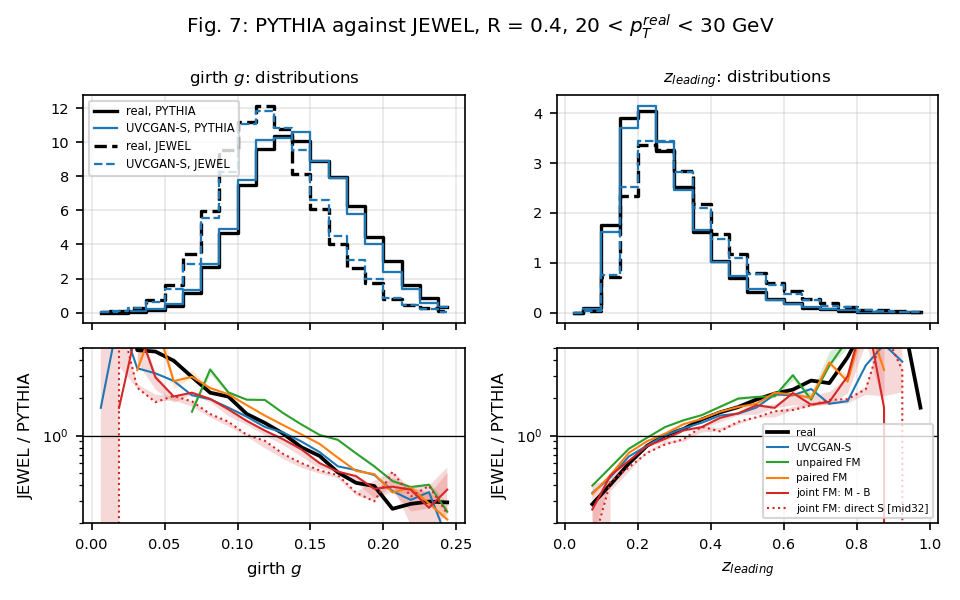
\includegraphics[width=\textwidth]{bench_fig7.png}
\column{0.56\textwidth}
\small
\begin{itemize}\setlength\itemsep{0.2em}
\item The PYTHIA calibration carries over with a +4\% shift for \uv{} and the background-only
  flows, +7-8\% for \jnt{}; calibrated resolution stays at 0.151-0.161.
\item \jnt{} ($M - \Bh$) does better on JEWEL than on PYTHIA (scale 0.98, per-jet girth error
  the smallest), consistent with its keeping hard towers: JEWEL jets are narrower.
\item \unp{}: fakes rise to 19\%. \pai{} keeps 0.72 of the girth shift (\uv{} 0.76), the others
  0.63; the mass shift is kept least (0.22-0.55).
\end{itemize}
\end{columns}
\vspace{0.1em}
\begin{center}
\scriptsize
\setlength{\tabcolsep}{4pt}
\begin{tabular}{lrrrrrrrr}
\toprule
 & scale & scale$_{cal}$ & res.$_{cal}$ & fake 14-20 & $g$ RMSE/$\sigma$ & $z_{lead}$ RMSE/$\sigma$ & $\Delta g$ kept & $\Delta z_{lead}$ kept \\
\midrule
\uv & 1.022 & 1.046 & 0.151 & 0.080 & 0.63 & 0.34 & 0.76 & 0.80 \\
\area & 0.904 & 1.016 & 0.269 & 0.231 & -- & -- & -- & -- \\
\unp & 1.033(1) & 1.040 & 0.151(1) & 0.189(2) & 1.02 & 0.53 & 0.63 & 0.71 \\
\pai & 0.863(2) & 1.040 & 0.158(1) & 0.015(1) & 0.66 & 0.36 & 0.72 & 0.80 \\
\jnt, $M - \Bh$ & 0.981(14) & 1.072(1) & 0.154(1) & 0.075(12) & 0.57(2) & 0.35(1) & 0.63(1) & 0.73(1) \\
\jnt, direct $\Sh$ (32) & 0.963(18) & 1.079(1) & 0.161(2) & 0.062(11) & 0.84(5) & 0.61(4) & 0.63(1) & 0.80(1) \\
\bottomrule
\end{tabular}
\par\vspace{0.15em}\snote{JEWEL, R = 0.4, $20 < p_T^{real} < 30$ GeV, raw; cal: each run's val (PYTHIA) calibration, frozen. Kept: the JEWEL$-$PYTHIA shift of the mean, as a fraction of the truth's (stat.\ error 0.03, 0.04). seed mean of 3; (n): seed half range in units of the last digit, shown where $\geq$ 1.}

\end{center}
\end{frame}

% ---------------------------------------------------------------- 7
\begin{frame}{Where the error goes: background-only flows put part of the jet core into $\Bh$}
\begin{columns}[T]
\column{0.52\textwidth}
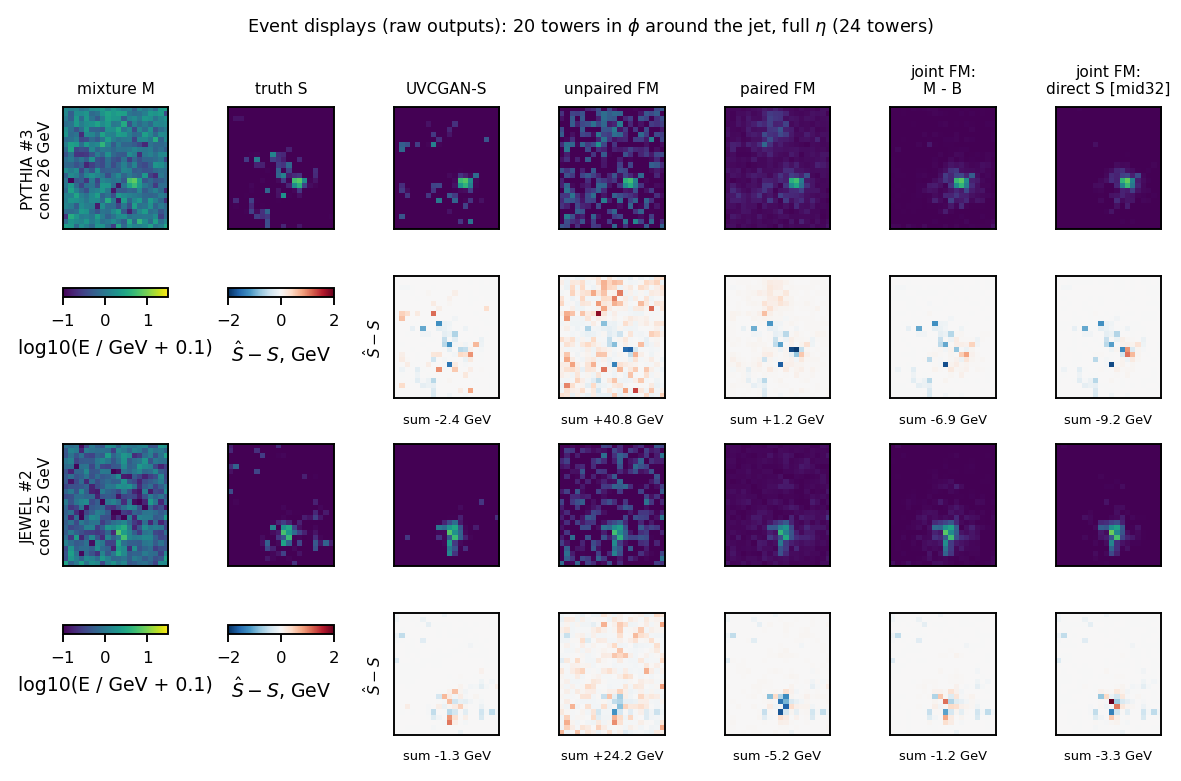
\includegraphics[width=\textwidth]{bench_displays.png}
\column{0.48\textwidth}
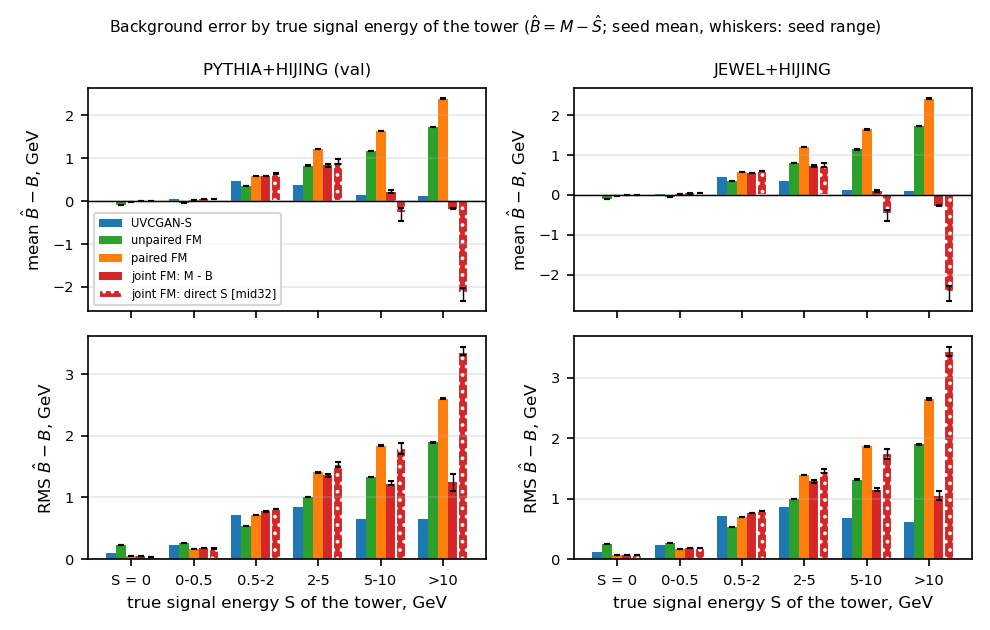
\includegraphics[width=\textwidth]{bench_bkgerr.png}
\tiny
\setlength{\tabcolsep}{3pt}
\begin{tabular}{lrrrr}
\toprule
 & MAE & \% $S$ lost, 5-10 & $>$10 GeV & $\sum(\Sh - S)$ \\
\midrule
\uv & 0.033 & 2 & 1 & -7 \\
\unp & 0.150 & 17 & 12 & 112 \\
\pai & 0.050 & 24 & 16 & 8 \\
\jnt, $M - \Bh$ & 0.031 & 3 & -1 & -19 \\
\jnt, direct $\Sh$ (32) & 0.031 & -4 & -14 & -25 \\
\bottomrule
\end{tabular}
\par\vspace{0.15em}\snote{val, raw; per tower (GeV), share of the true signal of towers with $S$ in 5-10 / $>$10 GeV put into $\Bh$, GeV per event; seed mean.}

\end{columns}
\vspace{-0.2em}
{\tiny Fixed events: the first of each set with a 25-35 GeV leading truth jet (the second:
\texttt{bench\_displays\_more.png}). In towers with $S < 2$ GeV every model misses 20-60\% of the
signal, \uv{} included (the 4-step \unp{} floor over-fills the softest).}
\end{frame}

% ---------------------------------------------------------------- 8
\begin{frame}{Conclusions}
\small
\begin{itemize}\setlength\itemsep{0.3em}
\item \textbf{Average resolution hides the failure modes.} \unp{} has the best cone resolution of the
  flows (3.67 GeV) and a jet scale of 0.99, yet puts 12\% of the hardest towers' energy into the
  background and adds a soft floor: 15\% fakes and the worst substructure distributions.
\item \textbf{Background-only vs joint (both paired, same budget): neither dominates.} Background-only
  keeps soft signal and gives the best per-jet substructure but loses 16-23\% of the hard core (scale
  0.83 / 0.75 by solver). Joint keeps the hard core but loses soft signal and low-$p_T$ jets, and varies
  more between seeds. With source $(M, 0)$ its signal channel reveals the answer for $t > 0$: the
  flow is decided in its first step (signal-channel loss 0.51 at $t = 0$, 0.0015 at $t = 0.02$).
\item \textbf{Pairing is not the fix for the core loss.} It improves images, fakes and per-jet
  substructure; the jet scale of background-only prediction stays low. It also needs per-mixture
  simulation truth.
\item \textbf{UVCGAN-S remains the reference for fidelity}, after ${\sim}$105 h and with its own supervised
  term. The flows train in 2 h and match its calibrated jet resolution, not its jet scale or distributions.
\item \textbf{Limits:} one network and 2-h budget for the flows; the analysis is rebuilt from the paper
  (no public code); ICS missing; \uv{} saw the val signal images in training (unpaired); the JEWEL
  sample's generator settings are not recorded.
\end{itemize}
\end{frame}

% ---------------------------------------------------------------- backup
\begin{frame}{Backup: both solves for every readout (same checkpoints)}
\scriptsize
\begin{tabular}{llrrrrrrrr}
\toprule
 & solve & cone res. & JEWEL & scale & res.$_{cal}$ & fake & $g$ RMSE/$\sigma$ & \% $S{>}10$ & MAE \\
\midrule
\unp & 4 Euler & 3.67$\pm$0.01 & 3.55$\pm$0.01 & 0.993(1) & 0.150 & 0.146(1) & 0.79 & 12 & 0.150 \\
 & 32 NFE & 4.10$\pm$0.01 & 3.65$\pm$0.01 & 0.742(2) & 0.155(1) & 0.002 & 0.53 & 24 & 0.051 \\
\addlinespace[0.2em] &  &  &  &  &  &  &  &  &  \\
\pai & 4 Euler & 3.95$\pm$0.00 & 3.61$\pm$0.00 & 0.828(2) & 0.154 & 0.005 & 0.55 & 16 & 0.050 \\
 & 32 NFE & 4.11$\pm$0.01 & 3.66$\pm$0.01 & 0.751(2) & 0.157 & 0.002 & 0.54 & 23 & 0.051 \\
\addlinespace[0.2em] &  &  &  &  &  &  &  &  &  \\
\jnt, $M - \Bh$ & 4 Euler & 4.15$\pm$0.04 & 4.12$\pm$0.05 & 0.912(16) & 0.161(3) & 0.029(3) & 0.68(4) & -1 & 0.031 \\
 & 32 NFE & 4.30$\pm$0.05 & 4.32$\pm$0.08 & 0.877(23) & 0.165(3) & 0.024(6) & 0.95(6) & -3 & 0.030 \\
\addlinespace[0.2em] &  &  &  &  &  &  &  &  &  \\
\jnt, direct $\Sh$ & 4 Euler & 5.80$\pm$0.25 & 5.19$\pm$0.19 & 0.780(18) & 0.174(5) & 0.004(1) & 0.86(4) & -13 & 0.033 \\
 & 32 NFE & 4.59$\pm$0.08 & 4.40$\pm$0.09 & 0.884(22) & 0.164(1) & 0.020(4) & 0.99(6) & -14 & 0.031 \\
\bottomrule
\end{tabular}
\par\vspace{0.15em}\snote{Cone res.: calibrated resolution in the true R = 0.4 cone, GeV (the selection metric), val and JEWEL, seed mean $\pm$ half range. Jets: R = 0.4, 20-30 GeV; fake 14-20 GeV; \% $S{>}10$: energy of towers with $S > 10$ GeV put into $\Bh$; MAE per tower, GeV. Seed 0 at 64 NFE, val cone res.: \unp{} 4.10, \pai{} 4.10, \jnt, $M - \Bh${} 4.34, \jnt, direct $\Sh${} 4.52. Joint $\Bh + \Sh - M$ before clean-up (val): 4 Euler: 0.009 GeV per tower (MAE), -7.7 GeV per event; 32 NFE: 0.003 GeV per tower (MAE), +1.3 GeV per event.}


\vspace{0.4em}
{\scriptsize
\begin{itemize}\setlength\itemsep{0.1em}
\item Val prefers 4 Euler steps for every readout except the joint direct $\Sh$ (32 NFE); the main
  slides use these. The accurate solve lowers the background-only jet scale further (0.83 $\to$ 0.75)
  and removes the unpaired floor (fakes 0.146 $\to$ 0.002): the floor is a 4-step artefact.
\item 32 NFE is resolved for the background-only flows (64 NFE: same val cone resolution to 0.01 GeV);
  for the joint direct readout 64 NFE changes it by 0.1 GeV.
\item Labelled clean-up (0.5 GeV tower threshold on every output) removes fakes but lowers every
  scale by a further 11-27\%; it does not restore the core (\texttt{bench\_summary.csv}, \texttt{[thr0.5]}).
\end{itemize}}
\end{frame}

\begin{frame}{Backup: comparability, limitations, what is missing}
\scriptsize
\begin{columns}[T]
\column{0.5\textwidth}
\textbf{Comparability}
\begin{itemize}\setlength\itemsep{0.1em}
\item Training time: flows 2 h (32k updates at batch 256); \uv{} ${\sim}$105 h (800k at batch 4). The
  equal-time view is \uv{} retrained from scratch: 8.4-16.7 h to 3.70 GeV, 6.9-8.6 GeV at 2 h.
\item Information: \pai{}, \jnt{} use each training mixture's true background; \uv{}'s \texttt{idt-aa} uses
  synthetic sums of independent $B$ and $S$; \unp{} uses no pairing. Same 633k mixtures for all flows.
\item One checkpoint per run, selected on val only (cone resolution, 4 Euler, $M - \Bh$); JEWEL never
  used for a choice. The paired arm's selected checkpoints are early (30-45 min): its cone resolution
  worsens with training while its per-tower error improves.
\item Statistical errors (one run) are shown apart from the seed spread (3 seeds).
\item Supplementary true-axis cone scores (\texttt{bench\_cone*.csv}): same ordering; the shape part of
  the EMD is smallest for \pai{} (2.93 GeV val) vs \uv{} 3.12.
\end{itemize}
\column{0.5\textwidth}
\textbf{Missing or limited}
\begin{itemize}\setlength\itemsep{0.1em}
\item ICS baseline: not available (fjcontrib not installed).
\item No public analysis code: tower threshold ($>0$), greedy matching, fake rate binned in
  $p_T^{sub}$, C/A soft-drop reclustering, jets $> 5$ GeV are our choices; Figs.\ 3-7 reproduced
  (\texttt{docs/flow/bench}), no paper numbers to compare.
\item The val events' signal images are among \uv{}'s (unpaired) training signals; HIJING parents of
  the embedded mixtures cannot be checked for train/val overlap (mixture keys are disjoint).
\item JEWEL sample (Zenodo 17594612): images only, generator version and settings not recorded
  (the paper states JEWEL 2.3.0 + Geant4).
\item Joint FM is still improving at 2 h; the budget is the same for all flows by design.
\end{itemize}
\end{columns}
\end{frame}

% ================================================================ follow-up
% Paired noisy-interpolant pilot (FLOW_NOTES.md, "Paired noisy-interpolant
% pilot"); numbers: docs/flow/bench/noisy/*.csv, tables/noisy_*.tex.

% ---------------------------------------------------------------- F1
\begin{frame}{Follow-up: does a noisy training path stop the paired flow's core leakage?}
\small
\textbf{The failure.} \pai{} background-only FM puts part of the jet core into $\Bh$ although every
training mixture comes with its own background: jet scale 0.83 (4 Euler) / 0.75 (accurate solve);
16\% / 23\% of the signal energy of towers with $S > 10$ GeV ends in $\Bh$. With $\Sh = M - \Bh$, lost
signal means $\Bh$ is \emph{too high}: the flow stops short of the true background in the core.

\vspace{0.3em}
\textbf{Hypothesis} (not an established explanation). Noiseless straight interpolants supervise the
velocity only on the segments between $(z(M), z(B))$ pairs; the states the ODE visits drift off them.
A noisy interpolant that returns exactly to the endpoints trains the field around the paths. Caveat: an
exactly learned marginal transport need not be the best estimator for single events.

\vspace{0.2em}
\begin{columns}[T]
\column{0.48\textwidth}
\footnotesize
\textbf{Path} (stochastic interpolant, Albergo, Boffi \& Vanden-Eijnden 2025), $a = z(M)$, $b = z(B)$:
\[ x_t = (1-t)\,a + t\,b + \eta \sin(\pi t)\,\varepsilon, \quad u_t = (b - a) + \eta\pi\cos(\pi t)\,\varepsilon, \]
the same $\varepsilon \sim N(0, I)$; $\eta$ = largest noise sd ($t = \tfrac12$), standardised $\log E$ units;
exact endpoints. Inference unchanged: deterministic ODE from $z(M)$, $\Sh = M - \Bh$.
\column{0.52\textwidth}
\footnotesize
\textbf{Controlled pilot} (seed 0): $\eta = 0$ against $\eta = 0.1$; same endpoint pairs, UVCGAN-S net,
633k mixtures, optimiser, EMA, readout; $\varepsilon$ from its own RNG (same weights, mixture order,
times); \textbf{32{,}640 updates each}, compared at the final update.
\begin{itemize}\setlength\itemsep{0.02em}
\item checks: $\eta = 0$ = old path bit for bit; exact endpoints; $u_t = \partial_t x_t$ to $3\cdot10^{-10}$;
  the fresh control repeats the benchmark run's loss curve
\item primary: accurate solve (midpoint 32 NFE; 64 checked); 4 Euler shown apart
\end{itemize}
\end{columns}
\end{frame}

% ---------------------------------------------------------------- F2
\begin{frame}{Pilot result: $\eta = 0.1$ changes nothing measurable (seed 0, 32{,}640 updates, val)}
\vspace{-0.5em}
\begin{columns}[T]
\column{0.56\textwidth}
\scriptsize
\setlength{\tabcolsep}{4pt}
\begin{tabular}{lrrrr}
\toprule
 & \multicolumn{2}{c}{32 NFE (accurate)} & \multicolumn{2}{c}{4 Euler} \\
 & $\eta = 0$ & $\eta = 0.1$ & $\eta = 0$ & $\eta = 0.1$ \\
\midrule
\% of $S$ in $\Bh$: $S > 10$ GeV & 23.1 & 23.2 & 15.8 & 15.9 \\
\hspace{1em}$S$ 5-10 GeV & 31.4 & 31.4 & 23.6 & 23.7 \\
\hspace{1em}$S$ 2-5 GeV & 47.0 & 47.0 & 39.4 & 39.6 \\
jet scale 20-30 & 0.753 & 0.753 & 0.832 & 0.831 \\
resolution (frozen cal.) & 0.161 & 0.161 & 0.156 & 0.157 \\
efficiency 14-20 & 0.956 & 0.959 & 0.969 & 0.971 \\
fake rate 14-20 & 0.002 & 0.002 & 0.006 & 0.005 \\
$\Bh - B$ at $S = 0$, GeV & -0.025 & -0.025 & -0.025 & -0.025 \\
$\sum(\Sh - S)$ / event, GeV & 0.7 & 0.7 & 6.1 & 6.0 \\
MAE / tower, GeV & 0.050 & 0.050 & 0.049 & 0.049 \\
\bottomrule
\end{tabular}


\vspace{0.4em}
{\scriptsize Substructure (per-jet RMSE$/\sigma$ and W1$/\sigma$ of $g, m, z_{lead}, p_T^D, z_g, r_g$):
$\eta = 0$ and $0.1$ agree to $\le 0.007\sigma$ at both solves (\texttt{noisy/noisy\_compare.csv}).
\uv{} for reference: scale 0.98, 0.8\% of the core in $\Bh$.}
\column{0.44\textwidth}
\vspace{-0.3em}
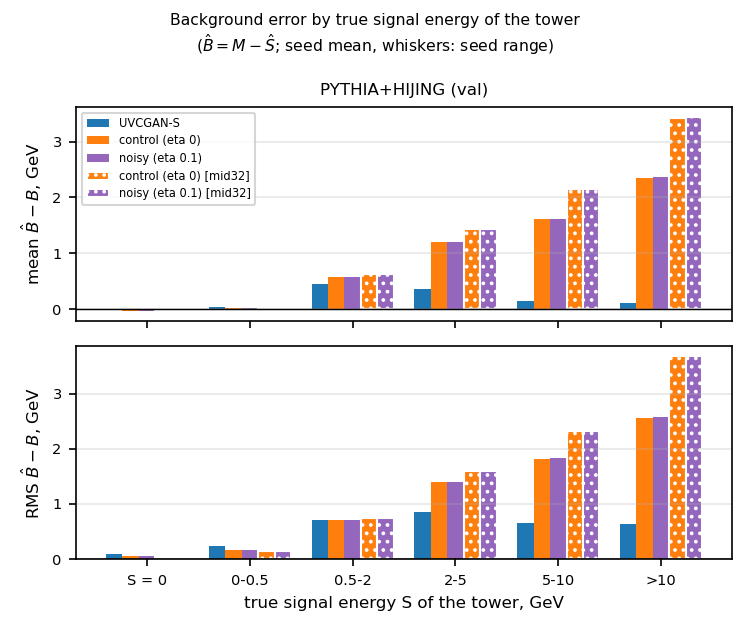
\includegraphics[width=\textwidth]{noisy/bench_bkgerr.png}
\end{columns}
\vspace{-0.2em}
{\scriptsize \textbf{All 58 pre-registered comparisons are within 3$\times$ the seed or statistical
spread} (largest core change $+0.0007$, threshold 0.0019). 64 NFE agrees with 32 to 0.0004 GeV per
tower. The 4-step readout keeps its trade-off in both arms: less core in $\Bh$, higher scale, +6 GeV
per event of spurious signal.}
\end{frame}

% ---------------------------------------------------------------- F3
\begin{frame}{Why not: the core stays in $\Bh$ even when the solve starts on the true path}
\vspace{-0.6em}
\begin{center}
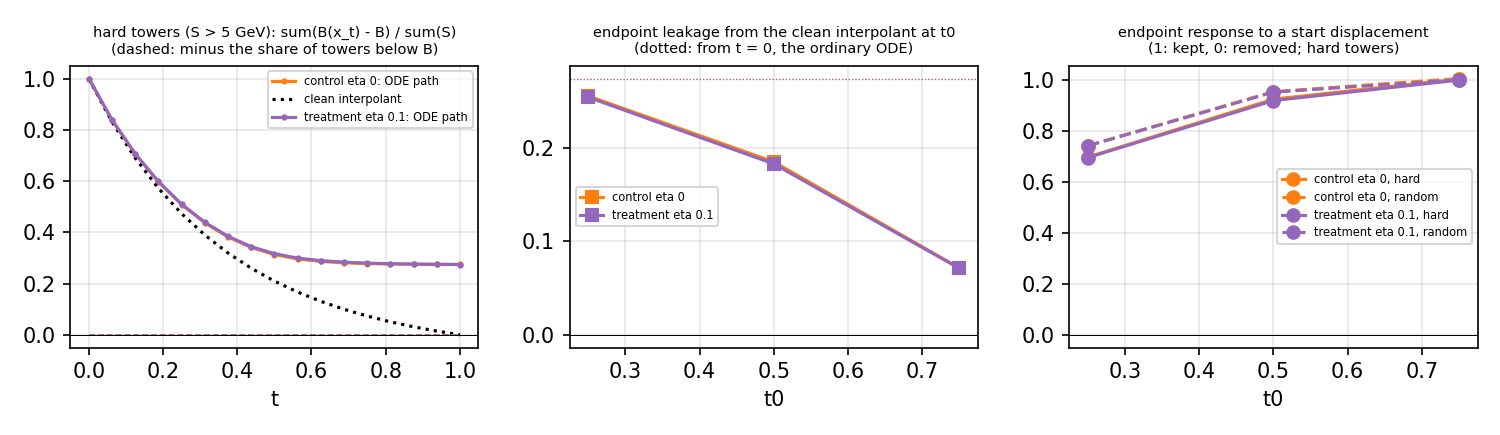
\includegraphics[width=0.92\textwidth]{noisy/traj.png}
\end{center}
\vspace{-0.9em}
{\scriptsize 256 val events, 592 towers with $S > 5$ GeV, final update, midpoint. Left: the ODE never
undershoots (no hard tower goes below the true $B$), follows the clean interpolant to $t \approx 0.2$
and stalls at 27\% after $t \approx 0.7$. Middle: started exactly on the true path at $t_0$, the rest of
the solve still leaves 26\% / 18\% / 7\% of the core in $\Bh$. Right: a displaced core is kept, not
restored. Both arms agree to 0.003.}

\vspace{0.2em}
\small
\textbf{Answer.} Noisy interpolation ($\eta = 0.1$) improved neither the accurately solved background
nor the jets, and did not shift the numerical trade-off either: both solves are unchanged. The loss
comes from the learned field on the paths, not from a lack of supervision around them
(hypothesis: the regression $E[b - a \mid x_t]$ averages over backgrounds the partly subtracted state
cannot tell apart). Pilot stopped: no seeds 1-2, no sweep, JEWEL untouched. This rules out only this
setting and says nothing about unpaired vacuum-to-medium transfer.
\end{frame}

\end{document}
